\documentclass{article}

\usepackage[OT1]{fontenc}
\usepackage{mathpazo}
\usepackage[italian]{babel}

\usepackage{amsmath}
\usepackage{amsfonts}
\usepackage[utf8]{inputenc}
\usepackage{graphicx}
\usepackage{float}
\usepackage{hyperref}
\hypersetup{
    colorlinks,
    citecolor=black,
    filecolor=black,
    linkcolor=black,
    urlcolor=black
}

\title{\textbf{Algoritmi Euristici}}
\author{Manuel Pagliuca}

\begin{document}

\maketitle
\tableofcontents

\section{Introduzione}
L'obiettivo di questo corso è quello di mostrare che gli \textbf{algoritmi euristici} non sono ricette per problemi specifici:
le euristiche e i problemi possono essere combinati liberamente.
Una qualsiasi euristica può essere utilizzata su un qualsiasi problema. \textit{Euristica} è una parola che deriva dal Greco,
e sta per \textit{"metodologia di ricerca della verità o dei fatti"}, deriva da \textit{heurìsko} che significa \textit{io trovo}.

Il termine deriva da una storia molto famosa di Archimede, che aveva da risolvere il problema di imparare se la data corona d'oro era effettivamente
d'oro o se fosse solo placcata in oro. Questo era possibile da dedurre conoscendo il rapporto tra peso e volume, però il peso era facile da ottenere,
mentre il volume è molto più difficile.

L'idea di Archimede consisteva nell'utilizzo di un secchio colmo di acqua ed immergendo la corona in quest'ultimo, il quantitativo di acqua che esce
dal secchio consiste nel volume della corona.
\section{Algoritmi euristici}
\subsection{Cenni sulla parola}
La parola \textit{euristica} può cambiare di significato in base al campo in cui viene utilizzata, in alcuni settori scientifici la parola \textit{algoritmo euristico}
è considerata come \textbf{ossimoro} in quanto le due parole vengono considerate opposti.
\begin{itemize}
    \item \textbf{Algoritmo} ha un significato che sta per \textit{procedura deterministica} e \textit{formale}, la quale consiste in una sequenza finita di step elementari.
    \item \textbf{Euristico} ha un significato che sta per \textit{informale, creativo} e \textit{metodo a "regola aperta"} per trovare una soluzione.
\end{itemize}

Ogni algoritmo ha (od è) una \textbf{dimostrazione di correttezza} mentre un algoritmo euristico non ne ha nessuna.
Essi sono trasformazioni meccanico-simboliche che partono da uno \textit{starting point} (chiamato \textit{ipotesi}) e giungono ad un \textit{end point}(chiamato \textit{tesi}).

\subsection{Definizione}
Gli algoritmi euristici sono procedure formali dove la soluzione non è garantita essere quella \textbf{corretta}. Questo potrebbe sembrare inutile,
ma al contrario potrebbe essere utile per diversi motivi:
\begin{enumerate}
    \item \textbf{Costa} molto meno di un algoritmo corretto, in termini di \textit{spazio} e \textit{tempo}.
    \item Frequentemente \textbf{restituisce} qualcosa di \underline{vicino} alla soluzione corretta.
\end{enumerate}

Per definire la \textit{vicinanza} della soluzione, lo \textbf{spazio delle soluzioni} sarà dotato di una \textit{metrica} per esprimere una \textit{distanza soddisfacente}
della soluzione corrente dalla soluzione corretta.
Inoltre sarà dotato di una \textbf{distribuzione probabilistica} per esprimere la frequenza soddisfacente delle soluzioni che si trovano ad una distanza soddisfacente dalla
soluzione corretta (ovvero esprime quanto spesso l'algoritmo restituisce una soluzione soddisfacente).

\subsection{Motivazioni per gli algoritmi euristici}
Le euristiche sono la costruzione sia delle \textbf{dimostrazioni} che degli \textbf{algoritmi}, in caso di successo l'euristica viene abbandonata e la
\textit{dimostrazione} viene preservata. Altrimenti, una buona euristica solitamente porta ad un buon risultato, seppur non perfetto.
\section{Classificazione dei problemi}
Questo corso è incentrato su gli algoritmi euristici applicati ai problemi di \textbf{ottimizzazione combinatoria} che sono \textbf{basati su soluzioni}
(contrapposti a quelli \textbf{basati sui modelli}).

Un problema è una domanda che viene effettuata su un \textbf{sistema matematico}, la tipologia dei problemi viene classificata in base alla natura delle loro soluzioni.
\begin{enumerate}
    \item \textbf{problemi di decisione}: la loro soluzione è un booleano.
    \item \textbf{problemi di ricerca}: la loro soluzione è un qualsiasi sottoinsieme \textit{fattibile}.
    \item \textbf{problemi di ottimizzazione}: la loro soluzione è un numero il quale è il \textit{minimo} o \textit{massimo} valore di una \textbf{funzione oggettiva}
          definita su dei sottoinsiemi fattibili.
    \item \textbf{problemi di conteggio}: la loro soluzione è il \textit{numero} di sottoinsiemi \textit{fattibili}.
    \item \textbf{problemi di enumerazione}: la loro soluzione è la collezione di tutti i sottoinsiemi \textit{fattibili}.
\end{enumerate}
I problemi di ottimizzazione possono essere combinati con i problemi di ricerca, noi ci concentreremo su questo tipo di problemi, ovvero siamo alla ricerca del
\textbf{valore ottimale} e del \textbf{sottosistema che assume} quel valore.

\subsection{Problemi di ottimizzazione e ricerca}

Un problema di ottimizzazione e ricerca può essere rappresentato con:
$$opt_{x\in X}f(x)$$
Dove $x$ rappresenta una \textbf{sottosistema fattibile} che è una delle soluzioni, la quale soddisfa le condizioni fornite dal problema. Invece, $X$
è lo \textbf{spazio delle soluzioni fattibili}. Invece la funzione, si chiama \textbf{funzione oggettiva} ed è mappata in questa maniera $f:X \rightarrow R$,
il suo compito è quello di \textit{misurare quantitativamente} la qualità di ogni sottosistema (o soluzione).
Generalmente, in quanto problema di ottimizzazione, la funzione oggettiva è \textit{massimizzabile} o \textit{minimizzabile}, questo viene denotato con $opt\in {min,max}$.

Il problema consiste nel determinare il \textbf{valore ottimale della funzione oggettiva} assieme alla \textbf{soluzione ottima} tale che sia un sottoinsieme. Il valore ottimale della funzione oggettiva viene chiamato $f^*$, ed è il risultato della seguente equazione:
$$f^*=opt_{x\in X}f(x)$$
Ovvero un valore che consiste nel minimo o massimo della funzione oggettiva. Mentre, la soluzione ottima tale che sia un sottoinsieme si chiamerà $x^*$:
$$x^*\in X^*=arg\textit{ } opt_{x\in X}f(x)={x^* \in X : f(x^*)=opt_{x\in X}f(x)}$$
Ovvero, vogliamo trovare una soluzione ottima nell'intero insieme di tutte le soluzioni ottime, anche se solitamente una è abbastanza, la notazione $arg$
sta per l'intero insieme delle soluzioni (ne basta una).

\subsection{Perchè siamo interessati nei problemi di ottimizzazione e ricerca ?}

I problemi di ottimizzazione e ricerca sono di forte interesse poiché diversi campi applicativi richiedono oggetti o strutture caratterizzati da valori molto alti o molto bassi rispetto ad una propria funzione di valutazione.
\begin{itemize}
    \item Bioinformatica
    \item Social networks
    \item Machine learning
    \item Hardware design
    \item Stima dei parametri
    \item Finanza
\end{itemize}

L'\textbf{ottimizzazione esatta} è costosa da un punto di vista computazionale e non sempre desiderabile (per questo gli algoritmi euristici sono favoriti);
perciò, solitamente, le funzioni di valutazione sono delle \textit{approssimazioni} di quello che realmente accade. In questo corso assumeremo il punto di vista dell'ottimizzazione, cercando di ottimizzare al meglio possibile la funzione oggettiva.

Diversi problemi possono spesso essere ridotti in problemi di ottimizzazione e ricerca
\begin{itemize}
    \item \textit{Problemi di ricerca} possono essere ridotti rilassando le condizioni da soddisfare, in maniera da allargare la \textbf{regione di fattibilità}
          da $X$ a $X'\supset X$ ed ottenere un problema di ricerca semplice. Si introduce una funzione $d(x)$ per quantificare la distanza di ogni soluzione $x\in X'$ da $X$. Infine, minimizzando $d(x)$ per trovare $x^*$ tale che $d(x^*)=0 \Leftrightarrow x^* \in X$.
    \item Alcuni \textit{problemi di decisione} riguardano l'esistenza di sottosistemi fattibili, e sono identici ai problemi di
          ricerca (trovare il sottosistema dimostra la sua esistenza).
    \item Alcuni \textit{problemi di numerazione} riguardano la richeca di sottosistemi con \textit{"buoni"} valori di funzioni oggettive in conflitto e permettono
          \textit{adattamenti diretti} ad algoritmi di ottimizzazione e ricerca.
\end{itemize}
Tali riduzioni sono spesso possibili ed utili, ma non sempre.

\subsection{Problema di ottimizzazione combinatoria (prima definizione)}
Un problema è un problema CO (\textit{Combinatorial Optimization}) quando la regione di fattibilità \textit{X} è un insieme finito, e quindi, che abbia un numero
finito di \textit{soluzioni fattibili}. Questa sembra un'assunzione molto restrittiva, ma sono presenti molti
problemi che hanno un numero infinito di soluzioni che possono essere ridotti a problemi che hanno un numero finito di soluzioni.

Per esempio:
\begin{itemize}
    \item I problemi infiniti nel discreto possono avere un insieme finito di soluzioni interessanti.
    \item Alcuni problemi continui possono essere ridotti a problemi di ottimizzazione combinatoria: \textit{Programmazione lineare, Flusso massimo, Costo minimo di flusso, ...}.
    \item I problemi continui possono essere ridotto in discreto utilizzando il campionamento (solitamente non è molto efficace).
    \item Le idee concepite per i problemi CO possono essere estese ad altri problemi.
\end{itemize}

\subsection{Euristiche basate sui modelli}
In questo corso parleremo solamente di \textbf{euristiche basate su soluzioni}, ma è importante conoscere anche la controparte.
L'euristiche basate sui modelli descrivono la regione di fattibilità $X$ con un "modello", un esempio tipico è una funzione matematica.
$$opt_{x\in X} f(x) \rightarrow \text{min}_{g_i(\xi)\leq 0}\phi(\xi) \text{ per } i=1,...,m$$

Dove $\xi \in \mathbb{R}^n$, il quale è il vettore delle soluzioni di $n$ numeri reali. Mentre $X={\xi \in \mathbb{R}^n : g_i(\xi)\leq 0, i=1,...,m}$, ovvero che la
regione di fattibilità è l'insieme dei vettori che soddisfanno tutte le disuguaglianze.
L'euristiche basate su modelli estrapolano l'informazione derivata dal modello, che sono le proprietà analitiche della funzione $\phi$ e $g_i \text{ per } i=1,...m$.

\subsection{Definizione alternativa di problema di ottimizzazione combinatoria}
Una problema è un problema CO quando:
\begin{enumerate}
    \item Il numero di soluzioni fattibili è finito (prima definizione).
    \item La regione di fattibilità è $X\subseteq 2^B$ per un dato \textbf{ground set} $B$, ovvero, le \textit{soluzioni fattibili} sono tutte sottoinsiemi del ground set che
          soddisfa le condizioni adeguate.
\end{enumerate}

Entrambe le definizioni sono equivalenti:
\begin{itemize}
    \item $2 \implies 1$: se il ground set $B$ è finito, ogni collezione $X\subseteq 2^B$ è finita.
    \item $1 \implies 2$: se il numero di soluzioni fattibili è finito, definire $B$ come il loro sovrainsieme ed $X$ la \textit{regione fattibile} sarà la
          collezione dei singoli elementi di $B$ (una \textit{"soluzione"} è un insieme contenente una singola soluzione).
\end{itemize}
In generale, la definizione sofisticata permette un analisi più profonda, perché $X$ non viene semplicemente numerato
e viene definito in una maniera \textit{compatta} e \textit{significativa}.

\subsection{Euristiche basate su soluzioni}
L'euristiche basate su soluzioni considerano le soluzioni come sottoinsiemi del ground set, esse possono essere classificate in:
\begin{enumerate}
    \item \textbf{Euristiche costruttive/distruttive}, iniziano da un sottoinsieme estremamente semplice
          (può essere $\emptyset$ o $B$), poi, esse aggiungono/rimuovono gli elementi fino a che non ottengono la soluzione desiderata.
    \item \textbf{Euristiche di scambio}, iniziano da un sottoinsieme ottenuto in una qualsiasi maniera,
          poi, scambiano gli elementi fino a che non ottengono la soluzione desiderata.
    \item \textbf{Euristiche di ricombinazione}, iniziano da una popolazione di sottoinsiemi ottenuta in una qualsiasi maniera,
          poi, ricombinando differenti sottoinsiemi produrranno una \textit{nuova} popolazione.
\end{enumerate}

I progettisti delle euristiche possono combinare in maniera creativa gli elementi delle diverse classi delle euristiche.

\subsubsection{Randomizzazione e memoria}
Sono presenti due cose importanti che intervengono nella progettazione di un algoritmo:
\begin{itemize}
    \item \textbf{Randomizzazione}
    \item \textbf{Memoria}
\end{itemize}

Puoi avere algoritmi che usano o non usano la randomizzazione o la memoria.
Questi due elementi sono ortogonali (indipendenti) rispetto alla classificazione delle eurisitche basate sulle soluzioni, per ognuna di esse possiamo dire che abbiamo quattro sottoclassi.

\begin{enumerate}
    \item Utilizzo della randomizzazione:
          \begin{itemize}
              \item \textbf{Euristiche puramente deterministiche}
              \item \textbf{Euristiche \textit{"randomizzate"}}, essenzialmente sono algoritmi che utilizzano come input numeri pseudo-casuali.
          \end{itemize}
    \item Utilizzo della memoria:
          \begin{itemize}
              \item Euristiche dove l'input include solamente i \textbf{dati del problema}.
              \item Euristiche dove l'input include anche \textbf{soluzioni precedentemente generate}.
          \end{itemize}
\end{enumerate}

Comunemente si utilizza il termine \textit{metaeuristiche} (dal Greco, \textit{"oltre le euristiche"}) per descrivere gli algoritmi euristici
che vanno utilizzano la randomizzazione e/o la memoria.

\subsection{Rischi da cui stare attenti}
\begin{enumerate}
    \item \textbf{Attitudine reverenziale o alla tendenza}, ovvero, nello scegliere un algoritmo basato sul contesto sociale, anziché sul problema.
    \item \textbf{Attitudine magica}, ovvero, \textit{credere} in un metodo sulla base di un analogia con un fenomeno fisico e naturale.
    \item \textbf{Integralismo euristico}, ovvero, utilizzare un euristica per un problema che ammette l'utilizzo di un algoritmo esatto.
    \item \textbf{Sgranocchiare numeri}, ovvero, performare sofisticati e complessi calcoli con numeri inaffidabili.
    \item \textbf{Attitudine SUV}, ovvero, affidarsi alla potenza dell'hardware.
    \item \textbf{Complicare ulteriormente}, ovvero, introdurre componenti e parametri \textit{ridondanti}, per cercare (fallendo) di migliorare il risultato.
    \item \textbf{Overfitting}, ovvero, adattare i componenti ed i parametri dell'algoritmo ad un dataset specifico utilizzato nella valutazione sperimentale.
\end{enumerate}

Inoltre è fondamentale:
\begin{itemize}
    \item Liberarsi dai pregiudizi.
    \item Valutare le prestazioni dell'algoritmo in una maniera scientifica.
    \item Distinguire il contributo di ogni componente dell'algoritmo.
    \item Implementare efficientemente ogni componente dell'algoritmo.
\end{itemize}

\section{Problemi di ottimizzazione combinatoria}
Il ground set è la base sul quale si costruisce l'algoritmo, abbiamo visto che sono presenti molteplici possibilità con le
euristiche basate sulle soluzioni, la loro classe cambierà in base al ground set utilizzato.
Quindi per prima cosa dobbiamo capire che cosa è (\textit{tipologia}) il \textbf{ground set}.

Visiteremo inizialmente un certo numero di problemi, questo sarà utile perché:
\begin{itemize}
    \item Le idee astratte devono essere applicate concretamente su diversi algoritmi per diversi problemi.
    \item La stessa idea può avere differente efficacia su diversi problemi.
    \item Alcune idee funzionano solamente su problemi con una specifica struttura.
    \item Diversi problemi potrebbero non avere un apparente relazione, cosa che può essere sfruttata per progettare algoritmi.
\end{itemize}

Una buona conoscenza di diversi problemi ci insegna ad applicare le idee astratte a nuovi problemi e ci insegna come trovare e sfruttare le relazioni tra problemi conosciuti e nuovi.

\subsection{Insieme dei problemi pesati}
\subsubsection{Knapsack Problem (KP)}
Il problema dello zaino, \textit{Knapsack Problem}. Il problema consiste nell'avere a disposizione uno zaino che ha una \textit{capacità limitata} ed un insieme di oggetti con differenti
\textit{volumi} e \textit{valori}, si vuole riempire lo zaino con gli oggetti di valore massimo (ovviamente non si può mettere dentro tutti gli oggetti).

Dati:
\begin{itemize}
    \item Insieme elementare $E$ di oggetti.
    \item Una funzione $v:E\rightarrow \mathbb{N}$ che descrive il \textbf{volume} di ogni oggetto.
    \item Un numero $V\in \mathbb{N}$ che descrive la \textbf{capacità} dello zaino.
    \item Una funzione $\phi : E\rightarrow \mathbb{N}$ che descrive il \textbf{valore} di ogni oggetto.
\end{itemize}

Banalmente, il \textbf{ground set} è l'insieme degli oggetti $B\equiv E$. La \textbf{regione di fattibilità} include tutti i sottoinsiemi degli
oggetti il cui volume totale non eccede la capacità $V$ dello zaino.
$$X=\left\{x\subseteq B : \sum_{j\in x}v_j \leq V\right\}$$

L'obiettivo è quello di massimizzare il valore totale degli oggetti scelti:
$$max_{x\in X} f(x)=\sum_{j\in x}\phi_j$$

Per esempio, nella seguente tabella sono mostrati tutti gli elementi di $E$ con i relativi valori e volumi. Sapendo che lo zaino ha una capacità massima $V=8$, consideriamo due \textbf{soluzioni candidate}:

\begin{figure}[H]
    \centering
    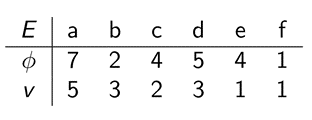
\includegraphics[width=6cm]{images/tab_KP.png}
    \caption{Dataset}
    \label{fig:tab_KP}
\end{figure}

\begin{figure}[H]
    \centering
    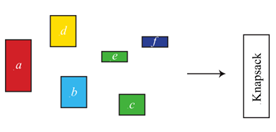
\includegraphics[width=6cm]{images/graphic_KP.png}
    \caption{Raffigurazione problema dello zaino}
    \label{fig:graphic_KP}
\end{figure}

\begin{figure}[H]
    \centering
    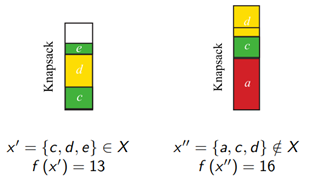
\includegraphics[width=8cm]{images/cand_sol_KP.png}
    \caption{Soluzioni candidate}
    \label{fig:cand_sol_KP}
\end{figure}

\begin{itemize}
    \item La prima soluzione candidata considera tre elementi la cui somma è $\leq V$, questo significa che la
          soluzione è un sottoinsieme preso dalla regione di fattibilità $X$ ed è una \textbf{soluzione fattibile}.
    \item La seconda soluzione candidata ha una somma di elementi pari a $10$, la quale è $>V$. Quindi questo sotto insieme
          non è appartenente alla regione di fattibilità $X$ (ma solo al ground set), perciò verrà chiamata \textbf{soluzione infattibile}.
\end{itemize}

Tra le soluzioni fattibili proposte la \textbf{funzione oggettiva} propone di prendere la soluzione \textit{massima}, ma visto che $x''$ non è fattibile, prenderemo come soluzione $x'$.
\subsubsection{Maximum Diversity Problem (MDP)}
Il problema della diversità massima, \textit{Maximum Diversity Problem}, è un problema importante per il corso e
verrà utilizzato come esempio per la parte di laboratorio. Questo è un problema
definito su uno spazio metrico, quindi uno spazio con la nozione di \textit{distanza}.

Dati:
\begin{itemize}
    \item Un insieme di punti $P$.
    \item Una funzione $d:P \times P \rightarrow \mathbb{N}$, la quale provvede la distanza tra le coppie di punti.
    \item Un numero $k\in {1,...,|P|}$, il quale è il numero di punti che si vuole selezionare.
\end{itemize}

Il problema chiede di selezionare da un insieme di punti $P$ un sottoinsieme di $k$ punti la cui sommatoria delle distanze tra le coppie dei punti sia massima.
Questo è un problema CO, perchè il numero di sottoinsiemi possibili è finito, ed in particolare è un problema CO perché le soluzioni sono sottoinsiemi del ground set.
Il ground set, banalmente, è l'insieme dei punti $B\equiv P$, mentre la regione di fattibilità include tutti i sottoinsiemi composti da $k$ punti.
$$X=\left\{x\subseteq B : |x| = k \right\}$$
La funzione oggettiva è la sommatoria di tutte le distanze tra le coppie di punti in $x$:
$$max\underset{x\in X}{f(x)}=\sum_{(i,j):i,j\in x}d_{ij}$$

Per esempio, consideriamo un dataset costituito da $7$ punti e considerando un $k=3$, questo significa che vogliamo trovare
un sottoinsieme costituito da $3$ punti tale che le coppie abbiano distanza massima.

\begin{figure}[H]
    \centering
    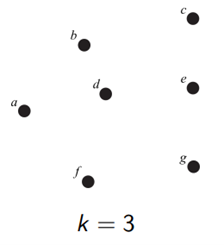
\includegraphics[width=3cm]{images/graph_MDP.png}
    \caption{Dataset}
    \label{fig:graph_MDP}
\end{figure}

\begin{figure}[H]
    \centering
    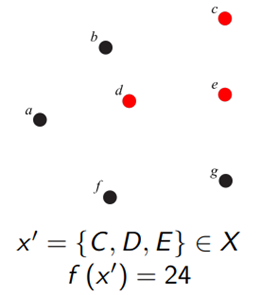
\includegraphics[width=3cm]{images/sol1_MDP.png}
    \caption{Prima soluzione candidata del MDP}
    \label{fig:cand_sol_MDP}
\end{figure}

\begin{figure}[H]
    \centering
    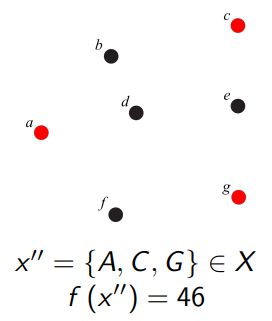
\includegraphics[width=3cm]{images/sol_MDP.png}
    \caption{Seconda soluzione candidata del MDP}
    \label{fig:cand_sol_2_MDP}
\end{figure}

La prima soluzione $x'$, considerando una metrica \textit{non fornita} ha come valutazione della funzione oggettiva $f(x')=24$, ed è un sottoinsieme tale per cui
la sua cardinalità sia $\leq k$, e quindi appartenente alla regione di fattibilità $X$.

La seconda soluzione ha come soluzione della funzione oggettiva $f(x'')=46$, questo è anche fattibile visto che $|x''|=k$, ed è una soluzione preferibile alla prima visto che
stiamo cercando il sottoinsieme che soddisfi massimo della funzione oggettiva.

\subsubsection{Interludio 1: la funzione oggettiva}
Fermiamoci un attimo e pensiamo qualcosa a riguardo di questo problema, in particolare soffermiamoci sulla funzione oggettiva.
Questa viene data come funzione che ha come dominio la regione di fattibilità e giunge al
codominio all'insieme dei numeri naturali.
$$f:X\rightarrow \mathbb{N}$$

Il calcolo di questa funzione potrebbe essere molto complesso ed estenuante, ogni singola soluzione ha il proprio valore rispetto alla funzione oggettiva
e si dovrebbe andare a controllare ogni volta in una tabella per svolgere il calcolo, non è una cosa molto interessante da fare.

Questo ovviamente, non è il caso dei precedenti problemi in quanto semplici da svolgere.

In particolare il problema KP una funzione oggettiva \textbf{additiva}, nel calcolare la $f$ dobbiamo effettuare delle somme
con il valore della funzione ausiliaria $\phi$ definita sul ground set, ricordando che nel problema KP, $B \equiv E$.
$$\phi : B\rightarrow \mathbb{N} \text{ induce } f(x)=\sum_{j\in x}\phi_j : X \rightarrow \mathbb{N}$$

Questo è interessante perchè significa che si deve memorizzare solamente il valore della funzione ausiliaria $\phi$, i quali sono $|B|$ valori, e non $2^B$, come
sarebbe per i valori della funzione oggettiva che è definita su $X$.
\newline
\newline
Lo stesso accade per il problema MDP e la sua funzione ausiliaria $d$, anche se quest'ultima ha una funzione oggettiva quadratica,
poi fornito un $n=|B|$ di punti nel caso peggiore si dovranno sommare $\frac{n(n-1)}{2}$ (numero di archi in un grafo completo) distanze, tuttavia però il
calcolo rimane \textit{"solamente"} una somma, quindi avente una \textbf{complessità polinomiale}.
\newline
Nel problema KP una volta che il valore viene fornito per uno specifico sottoinsieme, rimane possibile modificare gli elementi
e ricalcolare il valore della funzione oggettiva facilmente. Il valore della funzione oggettiva nel caso del MDP va trattato in maniera differente
per essere calcolato in tempo lineare (poiché quadratica).

Un'altra importante osservazione è che il problema KP e MDP sono definiti sull'intero insieme delle possibili (non fattibili)
soluzioni $2^B$, e questo è generalmente inutile visto che stiamo cercando
una soluzione fattibile (in alcuni casi questo però sarà utile).

Per riassumere, quando guardiamo un problema cerchiamo di capire come la funzione oggettiva è costituita:
\begin{itemize}
    \item È una funzione additiva?
    \item È una funzione quadratica?
    \item È una funzione semplice da calcolare?
    \item È una funzione semplice da aggiornare?
    \item Su cosa è definita la funzione oggettiva?
\end{itemize}

\subsection{Insieme dei problemi di partizionamento (BDP)}
In questi problemi un insieme di oggetti viene fornito, l'obiettivo consiste nel dividerlo in sottoinsiemi ottenendo una partizione con alcune peculiarità.
\subsubsection{Bin Packing Problem (BPP)}
Il Bin Packing Problem (BPP), si ha un insieme di oggetti con un \textit{volume}, e si vuole mettere questi oggetti all'interno di
container con una \textit{capacità fissa} (fornita) utilizzando il \textbf{minimo numero di container}.

Dati:
\begin{itemize}
    \item Insieme $E$ di oggetti.
    \item Una funzione $v:E \rightarrow \mathbb{N}$ che fornisce il volume per un dato oggetto $e\in E$.
    \item Un insieme $C$ di containers.
    \item Un numero $V\in \mathbb{N}$ il quale rappresenta la capienza massima dei container (volume massimo contenibile).
\end{itemize}

La prima domanda che ci si vuole porre è: \textit{è un problema di ottimizzazione combinatoria?}

Il ground set è definito come $B=E\times C$, dove ogni elemento di $B$ è definito da una coppia $\langle oggetto, container\rangle$. Una soluzione
per questo problema è un sottoinsieme formato da oggetti di questo tipo, il prodotto cartesiano è necessario poichè si deve selezionare un oggetto ed inserirlo in un determinato container.

Una volta che la lista di coppie contenenti gli elementi di $E$
è costruita, una soluzione candidata sarà ottenuta (un sottoinsieme del ground set,
ma a noi questo non basta, voglia che sia un sottoinsieme della regione di fattibilità).
\newline
\newline
Consideriamo $B_e$ come il sottoinsieme del ground set dove gli oggetti delle coppie provengono da $E$ (i container sono tutti i possibili), e $B_c$ come il sottoinsieme del ground set dove i container nelle coppie degli elementi provengono da $C$ (gli elementi sono tutti i possibili).
$$B_e=\{(i,j) \in B : i=e\}$$
$$B_c=\{(i,j) \in B : i=c\}$$

La \textbf{regione di fattibilità} include tutte le partizione degli oggetti tra i
container tale per cui non ecceda la capacità di un qualsiasi container.
$$X=\left\{ x\subseteq B : |x\cap B_e|=1\text{ } \forall e \in E, \sum_{(e,c) \in B^c} v(e)\leq V \text{ } \forall c\in C \right\}$$

La prima parte dell'espressione è un vincolo sul sottoinsieme delle soluzioni fattibili $x$, dice che l'intersezione tra il sottoinsieme delle soluzioni fattibili ed il ground set deve avere modulo $1$. Questo significa che gli elementi
all'interno di $x$ devono essere presenti solamente una volta rispetto a gli elementi $E$ del ground set, ovvero $\in B_e$.

La seconda parte dell'espressione anch'essa è un vincolo ma rispetto al volume massimo dei container, dice che la somma dei volumi
di ogni singolo elemento del sottoinsieme fattibile non deve eccedere la capacità massima dei container $V$.

L'obiettivo è quello di minimizzare il numero di container utilizzati:
$$min\underset{x\in X}{f(x)}=|{c \in C : x\cap B^c \neq \emptyset}|$$

Per esempio, consideriamo degli oggetti con diversi volumi e sia data una capacità massima dei container pari a $V=4$.

\begin{figure}[H]
    \centering
    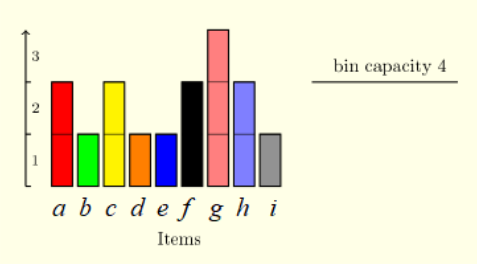
\includegraphics[width=6cm]{images/grap_BPP.png}
    \caption{Dataset}
    \label{fig:grap_BPP}
\end{figure}

\begin{figure}[H]
    \centering
    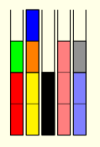
\includegraphics[width=2.5cm]{images/sol1_BPP.png}
    \caption{Prima soluzione candidata del Bin Packing Problem}
    \label{fig:sol1_BPP}
\end{figure}

Consideriamo la prima soluzione proposta, visto che la lista dei prodotti cartesiano
rispetta i due vincoli nella definizione della regione
di fattibilità la soluzione $x'$ è una \textbf{soluzione fattibile}.
$$x'=\{(a,1),(b,1),(c,2),(d,2),(e,2),(f,3),(g,4),(h,5),(i,5)\}\in X$$
$$f(x')=5$$

\begin{figure}[H]
    \centering
    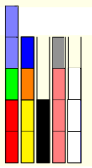
\includegraphics[width=2.5cm]{images/sol2_BPP.png}
    \caption{Seconda soluzione candidata del Bin Packing Problem}
    \label{fig:sol2_BPP}
\end{figure}

Invece, la seconda soluzione proposta è una \textbf{soluzione infattibile}, questo perché gli elementi non stanno
rispettando il secondo vincolo sul volume, e quindi
questo sottoinsieme non è compreso all'interno della regione di fattibilità.
$$x''={(a,1),(b,1),(c,2),(d,2),(e,2),(f,3),(g,4),(h,1),(i,4)}\notin X$$
$$f(x'')=4$$
Considerando il caso in cui $x''$ fosse una soluzione fattibile avremmo scelto quella tra le soluzioni
proposte, poiché la funzione oggettiva effettua l'ottimizzazione sul minimo.

\subsubsection{Parallel Machine Scheduling Problem (PMSP)}
Il Parallel Machine Scheduling Problem (PMSP), è un problema nel quale un insieme di attività (tasks) deve essere diviso lungo un set di macchine in modo che
il \textit{tempo di completamento} sia minimizzato.

Dati:
\begin{itemize}
    \item Un insieme $T$ di tasks (o \textit{attività}).
    \item Una funzione $d:T \rightarrow \mathbb{N}$ che descrive la lunghezza (temporale) di ogni task.
    \item Un insieme di $M$ macchine.
\end{itemize}

Come prima, il ground set è dato dal prodotto cartesiano di due set forniti:
$$B\equiv T\times M$$
Significa che la soluzione deve essere una coppia $$\langle task,macchina\rangle$$. È importante
sottolineare che la sequenza in cui i task sono eseguiti non è rilevante, invece è rilevante il \textbf{tempo di completamento}
, ovvero il tempo con cui l'ultimo task termina (o il tempo in cui una macchina completa l'esecuzione dei suoi tasks).

La regione di fattibilità include tutte le partizioni delle attività nella macchine:
$$X=\left\{ x\subseteq B : |x\cap B_t|=1 \text{ } \forall t \in T \right\} $$
La \textbf{funzione oggettiva} ha come obiettivo quello di minimizzare il massimo della sommatoria delle lunghezze di tempo per ogni task di ogni macchina:
$$min\underset{x\in X}{f(x)}=max\underset{m\in M}{}\sum_{t:(t,m)\in x} d_t$$

In parole povere, vogliamo trovare il sottoinsieme $x$ che minimizza il tempo di completamento di ciascuna
macchina, dove il tempo di completamento per un singolo task è $\sum_{t:(t,m)\in x} d_t$.
\newline
\newline
Per esempio, consideriamo il seguente insieme di dati per tre macchine, $|M|=3$, e sette task differenti $|T|=7$.

\begin{figure}[H]
    \centering
    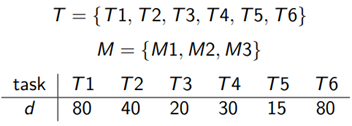
\includegraphics[width=5cm]{images/dataset_PMSP.png}
    \caption{Dataset del Parallel Machine Scheduling Problem}
    \label{fig:dataset_PMSP}
\end{figure}

\begin{figure}[H]
    \centering
    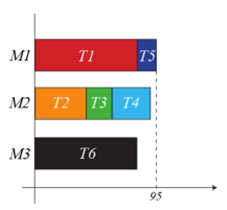
\includegraphics[width=4cm]{images/sol1_PMSP.png}
    \caption{Prima soluzione Parallel Machine Scheduling Problem}
    \label{fig:sol1_PMSP}
\end{figure}

Consideriamo la prima soluzione proposta:
$$x'={(T1,M1),(T2,M2),(T3,M2),(T4,M2),(T5,M1),(T6,M3)}\in X$$
$$f(x')=95$$
Possiamo notare che questa è una \textbf{soluzione fattibile},
visto che ogni task accade al meno ed al massimo una volta.
Notiamo che il valore assunto dalla funzione oggettiva è $95$, questo proprio
perché l'ultimo task ha un tempo di completamento pari a $95$.

\begin{figure}[H]
    \centering
    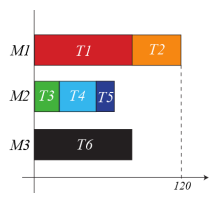
\includegraphics[width=4cm]{images/sol2_PMSP.png}
    \caption{Seconda soluzione Parallel Machine Scheduling Problem}
    \label{fig:sol2_PMSP}
\end{figure}

Consideriamo la seconda soluzione proposta:
$$x''={(T1,M1),(T2,M1),(T3,M2),(T4,M2),(T5,M2),(T6,M3)}\in X$$
$$f(x'')=120$$
Notiamo che anche questa è una \textbf{soluzione fattibile} visto che ogni task accade al
minimo ed al massimo una volta, in questo casa la funzione oggettiva assume come valore $120$.
Questo significa che fra le due soluzioni proposte la prima è quella \textbf{ottima}.

\subsubsection{Interludio 2: la funzione oggettiva, ancora}
È necessario familiarizzare con il fatto che il ground set $B$ non è sempre uno degli insiemi
forniti nel problema, ma può essere formato dalla combinazione (come il prodotto cartesiano)
di diversi insiemi forniti. Ora affrontiamo la domande proposte nell'ultimo interludio.

\textit{Le funzioni oggettivi di che tipo sono? (addittive, quadratiche,...)}
Questa volta le funzioni oggettive per il BPP e PMSP \textbf{non} sono additive, e non sono neanche banali.
È presente un algoritmo polinomiale per calcolare la funzione oggettiva, seppur non complesso,
non è semplice come per i problemi precedenti.

Notiamo che piccole modifiche alle soluzioni hanno un impatto \textit{variabile} sull'obiettivo, per esempio
consideriamo la seconda soluzione $x''$ del PMSP:
\begin{itemize}
    \item Spostare il task $T5$ sulla macchina $M1$, allunga il tempo di completamento complessivo$M1$,
          il risultato della funzione oggettiva cambia perché viene incrementato del task spostato (\textit{\textbf{impatto corrispondente al tempo del task spostato}}).
    \item Spostare il task $T5$ sulla macchina $M3$, non modifica il tempo di completamento complessivo
          delle macchine, il risultato della funzione oggettiva rimane lo stesso (\textit{\textbf{impatto zero}}).
    \item Spostare il task $T2$ sulla macchina $M2$, comporta una modifica dei tempi di completamento
          complessivi, il risultato della funzione oggettiva cambia poiché l'ultimo task viene spostato (\textit{\textbf{impatto intermedio}})

\end{itemize}

In fatti, l'impatto di una modifica di una soluzione dipende :
\begin{itemize}
    \item Da entrambi gli elementi modificati.
    \item E dagli elementi non modificati (questo è contrario alle cose dette nell'interludio 1).
\end{itemize}

Un punto interessante è che la funzione oggettiva del PMSP tende ad essere \textbf{piatta}, ovvero che sono presenti
molteplici soluzioni all'interno del problema dove il valore della funzione rimane lo stesso anche se avvengono
delle modifiche (l'esempio precedente, la soluzione $x''$ rimane fissa per diverse combinazioni su $120$).

\subsection{Problemi delle funzioni logiche}
\subsubsection{The Max-SAT problem}
Il problema del Max-Sat, sia da una formula in \textbf{forma normale congiuntiva}
(CNF, \textit{Conjunctive Normal Form}), si vogliono fornire in ingresso dei valori di
verità alle variabili logiche della CNF tali per cui la formula venga
soddisfatta (valutata come vera).

Dati:
\begin{itemize}
    \item Un insieme $V$ di \textbf{variabili logiche} $x_j$ con valori in $\mathbb{B}\in \{0,1\}$.
    \item Un \textbf{letterale} $l_j(x)\in {x_j,\overline{x}_j}$ che è una funzione che consiste in una variabile logica
          \textit{affermata} o \textit{negata}.
    \item Una \textbf{formula logica} $C_i(x)=l_{i,1} \lor ... \lor l_{i,n_i}$, la quale è
          una disgiunzione o \textit{somma logica} (OR) di lettarali. Soddisfare una formula
          logica significa fargli assumere valore 1.
    \item Una formula in \textbf{forma normale congiuntiva} $CNF(x)=C_1\land ... \land C_n$ è una congiunzione di \textit{prodotti logici} di formule logiche.
    \item Una funzione $w$ che provvede dei \textit{pesi} per la formula CNF. La funzione associa ogni formula logica
          della CNF ad un rispettivo peso.
\end{itemize}

Visto che la soluzione consiste in un sottoinsieme caratterizzato dall'assegnamento
di valori di verità a variabili logiche, il \textbf{ground set} sarà il prodotto cartesiano
fra le variabili logiche e l'insieme dei numeri booleani:
$$B=V\times\mathbb{B}=\left\{(x_1,0),(x_1,1),...,(x_n,0),(x_n,1)\right\}$$

La \textbf{regione di fattibilità} è l'insieme delle soluzioni fattibili tali che una \textit{variabile}
venga considerata al più una volta. Essa include tutti sottoinsiemi costituenti
gli assegnamenti semplici che sono:
\begin{itemize}
    \item \textbf{completi}, ovvero che ad ogni variabile corrisponde \textit{almeno} un letterale.
    \item \textbf{consistenti}, ovvero che per ogni variabile corrisponde \textit{al massimo} un letterale.
\end{itemize}

$$X=\left\{x\subseteq B : |x\cap B_v|=1 \text{ }\forall v \in V \right\}$$
$$B_{xj}=\{(x_j,0),(x_j,1)\}$$

La \textbf{funzione oggettiva} (come sempre ottimizzata):
$$max\underset{x\in X}{f(x)}=\sum_{i:C_i(x)=1}w_i$$
L'obiettivo è quello di massimizzare il peso totale della \textit{formula logica soddisfatta}
segnata come $C_i(x)=1 \text{ per } i=1,...,n$ (dove $n$ è il numero di formule logiche presenti).

Consideriamo il seguente esempio:

$$V=\left\{x_1,x_2,x_3,x_4\right\}$$
$$L=\left\{x_1, \overline{x}_1, x_2, \overline{x}_3, x_3,\overline{x}_4, x_4\right\}$$
$$C_1=\overline{x}_1\lor x_2 \text{ ... } C_7=x_2$$
$$CNF = (\overline{x}_1\lor x_2 )\land (\overline{x}_1\lor x_3 )\land (\overline{x}_1\lor \overline{x}_3 )\land (\overline{x}_2\lor x_4 )\land (\overline{x}_2\lor \overline{x}_4 )\land x_1\land x_2$$
$$w_i=1 \forall C_i$$

Consideriamo adesso la seguente soluzione:
$$x=\left\{(x_1,0),(x_2,0),(x_3,1 ),(x_4,1)\right\}$$
La funzione oggettiva per questa soluzione assume valore $f(x)=5$, significa che soddisfa
$5$ formule delle $7$.

\textit{Risulta semplice trovare il valore della funzione oggettiva?} Non proprio, la complessità
della funzione oggettive è polinomiale

In caso di pesi uniformi sono presenti un campo ristretto di valori, che vanno da $0$ a $n$,
il numero di formule logiche, anche se sono presenti $2^|V|$ combinazioni che possono essere considerate.
\end{document}